\section{Time Systems Relevant for GPS}

	\subsection{Special and General Relativity}
	GPS positioning is one of the very few everyday events in which relativistic effects must be accounted for. The whole system is based on clocks, and those clocks are moving.
	
	All the clocks are in a gravitational field (of the Earth), so General Relativity is significant. The clock signal has a nominal frequency of 10.23 MHz. Actually, the exact frequency is 10.229 999 995 43 MHz to adjust for relativistic effects giving a frequency of 10.23 MHz seen from the user on the Earth.
	
	The satellite clock is moving with respect to the receiver clock, so time is dilated and Special Relativity enters. And the Earth is rotating; light follows a spiral path. We cannot perfectly synchronize the clocks!
	
	The Sagnac Effect from the rotation is also fascinating. It destroys Einstein Synchronization, which depends on a constant speed of light. That constancy is restricted to inertial frames (no relative acceleration). The rotation of the Earth means that clock A can be synchronized with B, and B with C, but clock C is not synchronized with A. So we need a universal time that goes at a different rate from local time. This coordinated Universal Time is maintained at the GPS control center in Colorado Springs.
	\subsection{GPS Time and Leap seconds}
	
	The fundamental time unit used in GPS is one SI second. The SI second was defined at the 13th general conference of the International Committee of Weights and Measures in 1967,as the " duration of 9 192 631 770 periods of the radiation corresponding to the transition between the two hyperfine levels of the ground state of the cesium 133 atom." The SI day is defined as 84400 SI seconds and the Julian century as 36525 SI days.
	
	Since the apparent revolution of the sun about the Earth is non-uniform (this follows from Kepler’s second law) a fictitious mean sun is defined which circles the Equator with uniform velocity. The hour angle of this fictitious sun is called universal time UT.
	
	The time epoch denoted by the Julian date JD is expressed by a certain number of days and fraction of a day after a fundamental epoch sufficiently in the past to precede the historical record. Date 0 was chosen to be at $12^h$ UT on January 1, 4713 BC. The Julian day number denotes a day in this continuous count, or the length of time that has elapsed at $12^h$ UT on the day designated since this epoch.
	
	JD is a large number so often it is replaced by the Modified Julian Day MJD:
	$$MJD = JD — 2 400 000.5.$$
	Hence J2000.0 = MJD 51544.5. A Modified Julian Day starts at midnight.
	
	Keeping time in the universe, and to approach completeness we describe leap seconds. The international atomic time scale (TAI) does not maintain synchronization with the solar day, since the Earth’s rotation rate is slowing by almost 1 s per year. The realisation of a mean solar time is called Universal Time (UT1). The Coordinated Universal Time (UTC) is tied to International Atomic Time (TAI) by an offset of integer seconds that is regularly updated to keep UTC close to UT1.
	
	Leap seconds are introduced by the IERS so that UTC does not vary from UT1 by more than 0.9s. (The International Earth Rotation Service is also responsible for maintaining continuity with earlier data collected by optical instruments.) DUT1 is the difference between UT1 — UTC broadcast with time signals to a precision of $\pm$0.1 s.
	
	The time signals broadcast by the GPS satellites are synchronized with the atomic clock at the GPS Master Control Station in Colorado. Global Positioning System Time GPST was set to $0^h$ UTC on January 6, 1980 but is not incremented by UTC leap seconds.
	Therefore, there is an integer-second offset of 19s between GPST and TAI such that
	$$GPST + 19 s = TAI.$$
	Table\ref{tab:9.2} shows a total of 15 leap seconds between January 6, 1980 and late 2011:
	$$GPST = UTC + 15 s.$$
	
	\begin{table}
		\centering
		\caption{Date of introduction of leap seconds to be added to UTC to get GPST}
		\label{tab:9.2}
		\begin{tabular}{cc}
			\hline Total number of leap seconds & Date introduced \\ 
			\hline  1 & 30 June 1982 \\ 
			  2 & 30 June 1983 \\ 
			  3 & 30 June 1985 \\ 
			  4 & 31 Dec. 1987 \\ 
			  5 & 31 Dec. 1989 \\ 
			  6 & 31 Dec. 1990 \\ 
			  7 & 30 June 1992 \\ 
			  8 & 30 June 1993 \\ 
			  9 & 30 June 1994 \\ 
			 10 & 31 Dec. 1995 \\ 
			 11 & 30 June 1997 \\ 
			 12 & 31 Dec. 1998 \\ 
			 13 & 31 Dec. 1999 \\ 
			 14 & 31 Dec. 2005 \\ 
			 15 & 31 Dec. 2008 \\ 
			\hline 
		\end{tabular} 
	\end{table}
	
	
	Along with GPST, from the very beginning was introduced the GPS week numbers. Since January 6, 1980 every week has its own number. These words are written on week 1625.Within the week, the concept of seconds of week (sow) is used. This number counts from midnight between Saturday and Sunday which is also the beginning of the GPS week.
	
	Furthermore for convenience the individual days of the week are numbered: Sunday 1,.Monday 2, Tuesday 3, Wednesday 4, Thursday 5, Friday 6, and Saturday 7.
	
	Professional GPS software uses the day of week for numerical reasons. The seconds of week may be as large as $7 \times 24 \times 60 \times 60 = 604 800 s$. In order to keep track of the mm in a point position we have to know time at the level of 0.01 ns. Using seconds of week with twelve decimals is beyond the limits of most computers. So either you may split the real number holding the seconds of week into an integer part and a decimal part or you may compute time in terms of GPS week number, day of week, and seconds of day.
	
	The M-file $gps\_time$ finds GPS time (week w and seconds of week sow):
	
	\begin{lstlisting} 
	t = julday(2011,3,2,10); % year, month, day, hour
	[w,sow] = gps_time(t)
	w = 1625
	sow = 295200
	\end{lstlisting}
	To avoid under-or overflow at the beginning or end of a week we use the M-file $check\_t$.
	
	\subsection{easy1}\label{subsec:easy1}
	
	Nearly any GPS processing starts with time issues, easyl shows how to convert an epoch given as year, month, day, hour, minute, and second to Julian day number, and finally to week and seconds of week (sow).Below we bring a sample in RINEX format of observations taken at site 247j:
	\begin{figure}
		\centering
		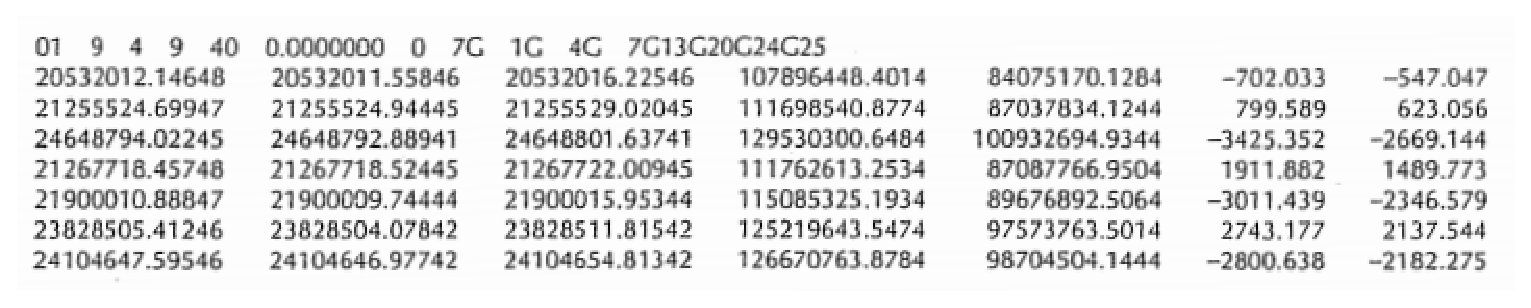
\includegraphics[width=0.7\linewidth]{TeX_files/Part03/chapter09/image/9-site247j}
	\end{figure}
	The first line of this data block tells the time of the epoch and pseudo random noise number of the satellites observed. We interpret that the epoch is from year 2001, month 9, day 4 at 9 hours and 40 minutes and 0 seconds. The following 0 indicates that the receiver is in static mode; next we read that 7 GPS satellites PRN 1, 4, 7, 13, 20, 24, and 25 are tracked.The next seven lines contain pseudorange and phase for those seven satellites: C/A code, P-code on L1 and L2, Phase on L1 and L2, and Doppler shifts on LI and L2.
	
	\subsection{Estimation of Receiver Clock Offset}
	
	Now we begin to use the data. First step is to estimate clock offsets $c\,dt_t$ .In GPS surveying, the code observations $b_t$ (pseudoranges) are often used to estimate the coordinates of a single point and the sequence of receiver clock offsets (changing with time). Suppose that epoch t contributes the linearized observation $b_t$:
	
	\begin{equation}\label{eq:9.1}
		A_t 
		\begin{bmatrix}
		x \\	y \\	z
		\end{bmatrix}
		+e_tcdt_t=b_t-\epsilon _t,\qquad t = 1,2,\ldots ,n.
	\end{equation}
	
	The matrix $A_t$ contains the partial derivatives of the observed pseudorange with respect to the coordinates at the epoch t. See (9.22) below. To add the clock error to each pseudorange, $e_t = (1, 1,\ldots ,1 )^T$ has m ones when there are m satellites in that epoch.We gather the observations from all n epochs into a unified least-squares problem
	
	\begin{equation}\label{eq:9.2}
		\begin{bmatrix}
		A_1 \\	A_2 \\	\vdots \\	A_n \\
		\end{bmatrix}
		\begin{bmatrix}
		x \\	y \\	z 
		\end{bmatrix}
		+		
		\begin{bmatrix}
		e_1 & & & \\
		& e_2 & & \\	
		& & \ddots & \\	
		& & & e_n  
		\end{bmatrix}
		\begin{bmatrix}
		c\,dt_1 \\	
		c\,dt_2 \\	
		\vdots \\	
		c\,dt_n
		\end{bmatrix}
		=\begin{bmatrix}
		b_1 \\ b_2 \\ \vdots \\ b_n
		\end{bmatrix}
		-
		\epsilon
	\end{equation}
	\begin{figure}
		\centering
		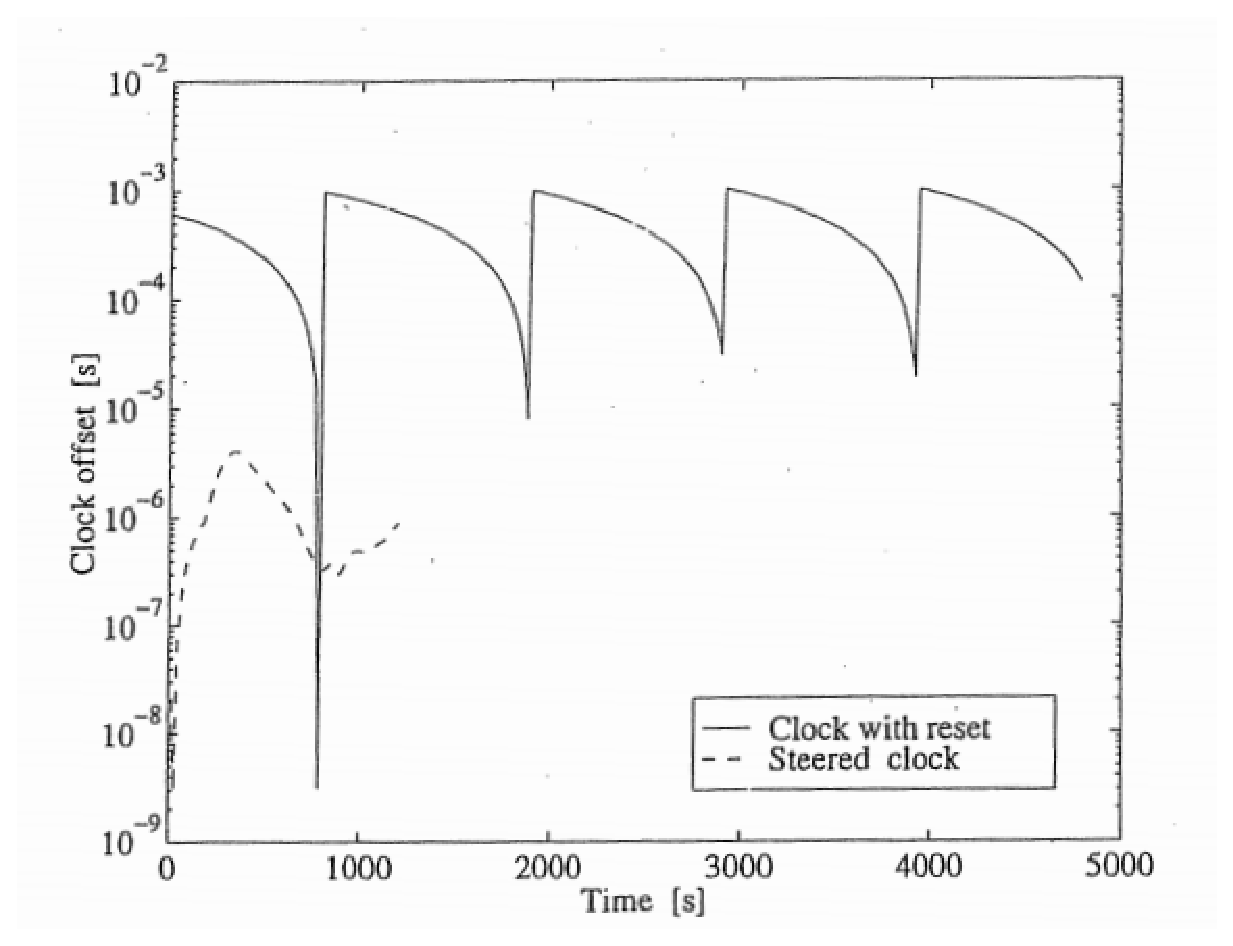
\includegraphics[width=0.7\linewidth]{TeX_files/Part03/chapter09/image/9-4}
		\caption{Offests for different receiver types.Theclock reset is 1ms.}
		\label{fig:9-4}
	\end{figure}

	The normal equations that solve \ref{eq:9.2} by least squares give the "best" x,y,z,$c\,dt_t$
	
	\begin{equation}\label{eq:9.3}
		\begin{bmatrix}
		e^T_1e_1 & & & & e^T_1A_1 \\
		& e^T_2e_2 & & & e^T_2A_2 \\
		& & \ddots   & & \vdots	  \\
		& & & e^T_ne_n & e^T_nA_n \\
		A^T_1e_1 & A^T_2e_2 & \ldots & A^T_ne_n & \Sigma ^n_{t=1}A^T_tA_t
		\end{bmatrix}
		\begin{bmatrix}
		c\,dt_1 \\
		c\,dt_2 \\
		\vdots
		c\,dt_n \\
		x \\
		y \\
		z 
		\end{bmatrix}
		=
		\begin{bmatrix}
		e^T_1b_1 \\
		e^T_2b_2 \\
		\vdots	 \\
		e^T_nb_n \\
		\Sigma ^n_{t=1}A^T_tb_t
		\end{bmatrix}
	\end{equation}
	
	By ordinary Gauss elimination we subtract multiples of the first n equations from the last block row. We write E t for the matrix$e_t(e^T_te_t)^{-1}e^T_t$ . The correction(x,y,z)of the preliminary position (X°, Y°, Z°) is determined by the matrix that appears in the lower right comer after elimination. According to (6.46) that corner yields
	$$x=\begin{bmatrix}
	x \\ y \\ z
	\end{bmatrix}=\left( \sum^n_{t=1}(A^T_tA_t-A^T_tE_tA_t)\right)^{-1}\sum^n_{t=1}(A^T_tb_t-A^T_tE_tb_t) $$
	The estimate of the receiver clock offsets c d t t is found by back substitution,$i=n,\ldots,1$:
	\begin{equation}
		c\,dt_t=(e_tb_t-e_tA_tx)/(e_te_t^T).
	\end{equation}
	
	The estimation model clearly demonstrates why it is not necessary to collect four observations at all epochs for static observations. But a sufficient number of observations is needed to keep \ref{eq:9.3} invertible. If only one observation is available at a particular epoch,we can estimate the receiver clock offset, but not the position.
	\begin{figure}
	\centering
	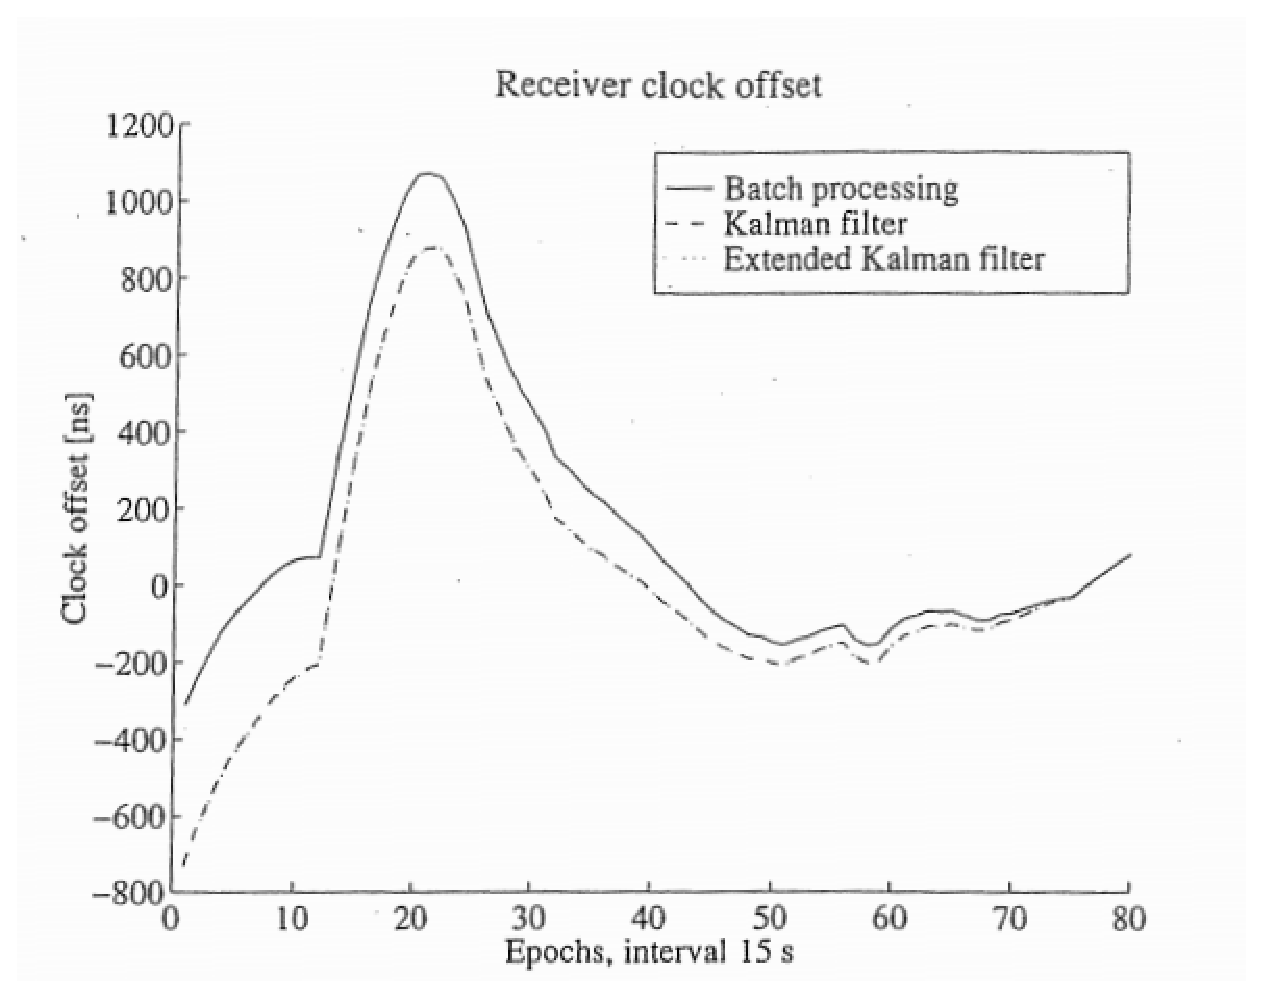
\includegraphics[width=0.7\linewidth]{TeX_files/Part03/chapter09/image/9-5}
	\caption{Receiver clock offsets computed by batch processing and Kalman filtering.The ordinary and extended Kalman filter coincide for linear processes}
	\label{fig:9-5}
	\end{figure}

	We recommend to use the described procedure, as some manufacturers introduce discontinuous changes in the clock time to keep the offsets within prescribed tolerances.Certain receivers have their clocks reset when the offset approaches one millisecond. Figure 9.4 demonstrates the jumps in the offset for this receiver type, as well as a receiver type which has a steered clock.Figure 9.5 shows the offset for a steered receiver clock with continual corrections to reduce the offset. The plot is made by the M-file recclock. The .code iterates three times to get the correct receiver position— the clock estimation is linear!
	
	\subsection{easy7}\label{subsec:easy7}
	
	The "pseudo" part of the word pseudorange alludes to the receiver clock offset dt. Most often dt is a parameter of less interest. However, in certain situations it is desirable to know dt . We apply the algorithm (9.4) to obtain dt. The actual data yield $dt\approx0.38 ms$ as shown in Figure 9.6. One can see that the rate of the receiver clock is fairly stable over a short period of time.
